\documentclass{beamer}
\usepackage{beamerthemeshadow}
\usepackage{graphicx}
\usepackage{color}
\usepackage[utf8]{inputenc}
\usepackage{hyperref}
\usepackage[flushleft]{threeparttable}
\usepackage{lipsum}
\usepackage{caption}
\usepackage{tabularx}
\usepackage{url}
\usepackage[english,serbian]{babel}
\definecolor{royalblue}{RGB}{26, 22, 130}
\setbeamercolor{structure}{fg=royalblue}

\title{Tehničko i naučno pisanje}
\subtitle{-- Stiven Hoking --}
\author{ Ivana Milenković\\ \and Lazar Rajčić\\ \and Anđela Spasić\\ \and Nikola Stanojević }
\institute{Matematički fakultet\\Univerzitet u Beogradu}
\date{
	\footnotesize{Beograd, 2022.}	
}

\begin {document}
\begin{frame}
	\thispagestyle{empty}
	\titlepage
\end{frame}

\addtocounter{framenumber}{-1}

\begin{frame}[fragile]\frametitle{Literatura}
	\begin{itemize} \fontsize{9}{6}\selectfont
		\item Zasnovano na:\\

	\item Stephen Hawking
	     \\ (\url{https://www.famousscientists.org/stephen-hawking/})
        \item  Stephen Hawking - British physicist
           \\ (\url{ https://www.britannica.com/biography/Stephen-Hawking})
        \item Stephen Hawking's Best Books: Black Holes, Multiverses and Singularities
           \\(\url{https://www.space.com/39987-stephen-hawking-best-books.html})
        \item Hawking's medals and awards
            \\(\url{ https://onlineonly.christies.com/s/shoulders-giants-newton-darwin-einstein-hawking/hawkings-medals-awards-50/62110})
       \item  Stephen Hawking
            \\(\url{ https://www.hawking.org.uk/biography})
        \item Stephen William Hawking CH CBE. 8 January 1942—14 March 2018
           \\ (\url{https://royalsocietypublishing.org/doi/10.1098/rsbm.2019.0001})
        \item J. Laski and W. Stanley. \emph{Software Verification and Analysis}. Springer- Verlag, London, 2009.
     \fontsize{6pt}{1pt}\selectfont
	\end{itemize}
\end{frame}

\begin{frame} \fontsize{9}{6}\selectfont
	\frametitle{Pregled}
	\tableofcontents[hidesubsections] 
\end{frame}
\section{Ko je Stiven Hoking?}

\begin{frame}[fragile]\frametitle{Ko je Stiven Hoking?}
	\begin{itemize} \fontsize{9}{6}\selectfont	
		\item  Stiven Hoking je bio engleski teoretski fizičar i kozmolog. Zbog njegovih doprinosa fizici smatran je za jednog od najvećih naučnika svog vremena. Njegovi doprinosi fizici se uglavnom nalaze u domenu našeg poznavanja crnih rupa. Zbog ovoga smatramo da je jako važno približiti njegova dostignuća ljudima.
\begin{figure}[h!]
  \centering
  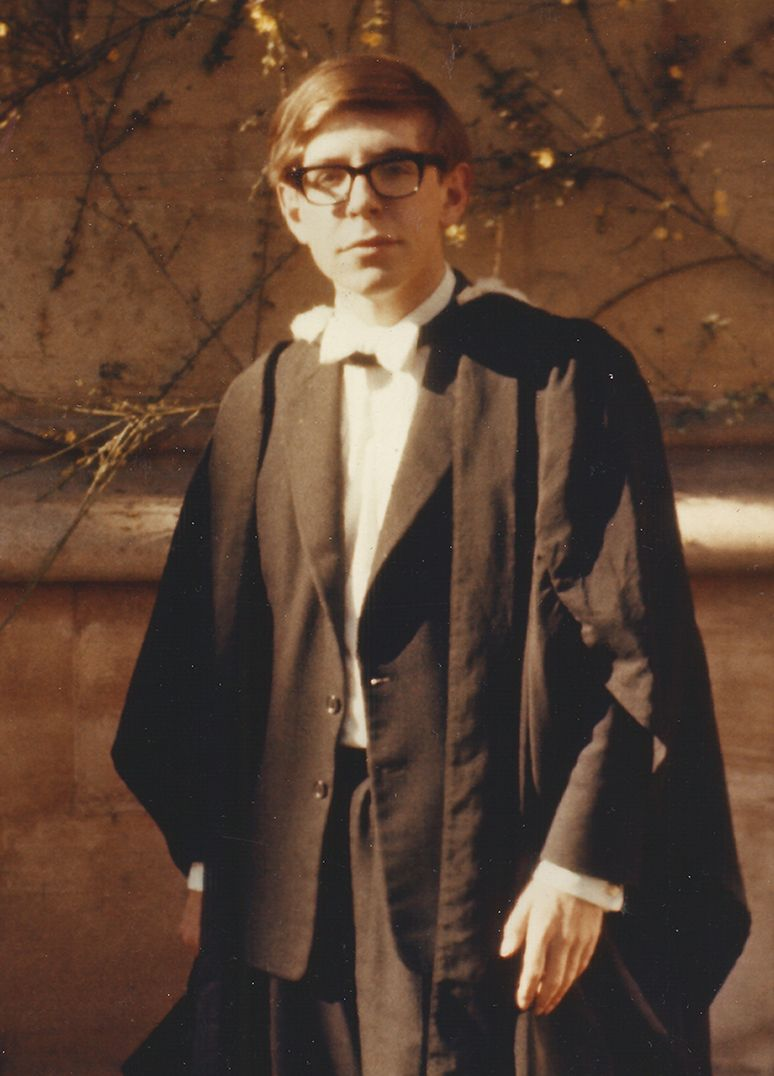
\includegraphics[width=0.3\textwidth]{Hoking,PreDijagnoze.jpg}
  \captionsetup{font=small}{Slika1: Hoking, na dodeli diploma 1960.}
  \label{fig:Hoking,PreDijagnoze}
  \end{figure}
	\end{itemize}
\end{frame}

\section{Život}
\begin{frame}[fragile]\frametitle{Rani život (Pre dijagnoze i dijagnoza)}
\begin{itemize}	 \fontsize{9}{6}\selectfont
		
\item  Hoking se rodio 8. Januara 1942. godine, tačno na tristotu godišnjicu smrti Galilea Galileja.
\item  U ranijim školskim godinama je dobio nadimak Ajnštajn.
\item  Zbog primedbi svog oca nastavio je da studira fiziku, a ne matematiku na Oksfordu. Osnovne studije je završio 1962. godine nakon čega prelazi na Kembridž univerzitet.
\item  Pri početku obrazovanja na Kembridžu primećuje kako je postao trapaviji. Nakon incidenta na klizanju odveden je u bolnicu na testiranje.
\item  Nedugo posle 21.-og rođendana saznaje da ima amiotrofičku lateralnu sklerozu (eng. Amyotrophic lateral 
sclerosis) skraćeno ALS. Uz dijagnozu su mu takođe rekli da neće živeti duže od još dve godine.
\item  Tek saznata vest ga demorališe ali uspeva ponovo da se pronađe u Vagnerovoj muzici i ljubavi prema Džejn Vajld.
\end{itemize}
\end{frame}
\begin{frame}[fragile]\frametitle{Život nakon dijagnoze}
	\begin{itemize} \fontsize{9}{6}\selectfont	
		\item  Nastavak svojih studija Stiven nije uspeo da pohađa pod Fredom Hojlom kao sto se tada nadao. 
		\item  Studije je nastavio pod Denisom Škiamom što se ispostavilo da je bilo bolje po njegovu karijeru. Škiam ga je upoznao sa Rodžerom Penrouzom sa kojim će kasnije sarađivati na jednom od svojih najvažnijih radova.
		\item  1965. godine neposredno nakon dobijanja doktorata Hoking stupa u bračnu zajednicu sa Džejn Vajld i prijavljuje se za istraživačku stipendiju.
		\item  U narednim godinama njegova bolest postaje sve ozbiljnija. Dolazi do tog nivoa da gubi mogućnost hoda kao i govora. Ovo uspeva da prevaziđe uz pomoc kolica i mašine koja sintetiše ljudski govor. 
		\item  Preminuo je u udobnosti svog doma, 14. marta 2018. godine. 
\begin{figure}[h!] 
\begin{center}
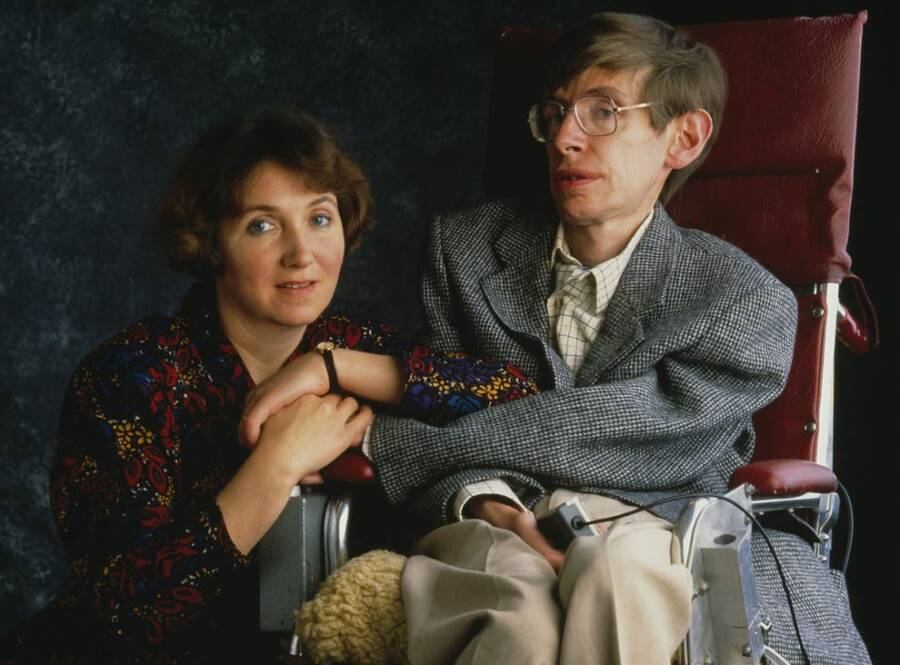
\includegraphics[width=0.3\textwidth]{StivenHoking.jpeg}
\end{center} 
 \captionsetup{font=small}{Slika2: Stiven Hoking i njegova žena} 
\label{fig:StivenHoking}
\end{figure}
\end{itemize}
\end{frame}


\section{Kariera}

\begin{frame}[fragile]\frametitle{Kariera}
\begin{itemize}	 \fontsize{9}{6}\selectfont
\item  Zvaničan početak njegove karijere označava godina 1965. Primarno je radio na poljima opšte relativnosti, posebno se interesujući za sferu crnih rupa.
\item Hoking je, 1970. godine zajedno sa Rodžerom Penrouzom dožao do veze između teorije relativiteta i velikog praska. Godinu dana kasnije dolazi do teorije malih crnih rupa, kojom je nađena veza između kvantne i klasične fizike, čije oktriće spada u jedno od Stivenovih najpoznatijih dela. Tri godine kasnije iznosi teoriju Hokingove radijacije. 
\end{itemize}
\end{frame}
\begin{frame}[fragile]\frametitle{Kariera}
	\begin{itemize}	 \fontsize{9}{6}\selectfont	
	\item  Osim toga što je bio teoretski fizičar i kosmolog, Hoking je takođe bio i autor, kao i član Kraljevskog društva (eng. Fellow of the Royal Society-FRS), doživotni član Papeške akademije nauka, dobitnik predsedničke medalje o slobodi, najviše civilne nagrade u SAD-u.	 Postao je profesor gravitacione fizike na Kembridžu 1977. godine, a 1979. je imenovan za Kembridžovog Lukasovskog profesora matematike (eng. Cambridges Lucasian professorship of mathematics), mesto koje je nekada imao Isak Njutn. Proglašen je za komandanta Ordena Britanske imperije 1982. godine i za Pratioca časti (eng. Companion of Honor) 1989. Takođe je dobio Koplei medalju (eng. Coplei medal) od Kraljevskog društva 2006. i Američku predsedničku medalju slobode 2009. Godine 2008. prihvatio je gostujuću istraživačku stolicu na institutu za teorijsku fiziku Perimeter u Kanadi.
	\end{itemize}
	\end{frame}
\section{Njegove najprodavanije knjige}

\begin{frame}[fragile]\frametitle{ Njegove najprodavanije knjige}
	\begin{itemize}	\fontsize{9}{6}\selectfont	
		\item Neke od knjiga koje je napisao a koje su se našle na listi najprodavajih su:
		\begin{itemize}\fontsize{9}{6}\selectfont
 \item Kratka povest vremena (1988) - upućena osobama koje nisu naučnici i proučava osnove univerzuma, kako je nastao i njegov mogući kraj
 \item Crne rupe i bebe vaseljene (1993) – skup Hokingovih eseja, od naučnih do privatnih
 \item Kosmos u orahovoj ljusci (2001) – nastavak na knjigu “Kratka povest vremena”, objašnjava pojmove kao što su supergravitacija, kvantna fizika, itd.
 \item Na plećima divova (2002) – pogled kroz radove Kopernika, Galilea, Keplera, Njutona i Ajnštajna
 \item Kraća povest vremena (2005) – dodatak na “Kratku povest vremena” i “Kosmos u orahovoj ljusci”
 \item Bog je stvorio cele brojeve: Matematički prodori koji su promenili istoriju (2005) –  prikazuje najvažnije delove istorije matematike, kao i biografije važnih matematičara
 \item Velika zamisao (2010) – opisuje poreklo univerzuma i prirodu realnosti, jedna od tema knjige su paralelni univerzumi
 \item Kratka istorija mog života (2013) – njegov memoar
\end{itemize}
\end{itemize}
\end{frame}	
	\section{Dostignuca}
	
	\begin{frame}[fragile]
	\vspace{1cm}
	\begin{table}[h!]
	\centering
	\caption{Nagrade koje je Stiven Hoking dobio tokom svog života.} 
	\medskip
	\resizebox{\columnwidth}{!}{%
	\begin{tabular}{|c|c|c|}
	\hline
	Godina & Nagrada & Razlog \\ \hline
	1975 & \begin{tabular}[c]{@{}c@{}}Edingtonova\\  medalja\end{tabular} & Za otkrića iz 1970. godine \\ \hline
	1976 & \begin{tabular}[c]{@{}c@{}}Medalja Džejms Klark fizičkog\\  instituta\end{tabular} & \begin{tabular}[c]{@{}c@{}}Za izvanredne rano-karijerske doprinose\\ teoretskoj fizici\end{tabular} \\ \hline
	1978 & \begin{tabular}[c]{@{}c@{}}Nagrada Albert \\ Ajnštajn\end{tabular} & Za uspeh u prirodnim naukama \\ \hline
	1979 & Medalja Društva Alberta Ajnštajna & \begin{tabular}[c]{@{}c@{}}Za naučne radove povezane sa Ajnštajnom\\ (Hoking je bio prvi primalac)\end{tabular} \\ \hline
	1985 & \begin{tabular}[c]{@{}c@{}}Zlatna medalja kraljevskog \\ astronomskog društva\end{tabular} & Za doprinose astronomiji \\ \hline
	1989 & Nagrada Britanika & \begin{tabular}[c]{@{}c@{}}Za širenje\\  znanja\end{tabular} \\ \hline
	1999 & \begin{tabular}[c]{@{}c@{}}Medalja društva umetničkih proizvođača\\ i trgovine\end{tabular} & \begin{tabular}[c]{@{}c@{}}Za činjenje fizike dostupnom i \\ razumljivijom\end{tabular} \\ \hline
	\end{tabular}%
	}
	\end{table}
	\end{frame}
	
	\section{Zakljucak}
	\begin{frame}[fragile]\frametitle{Zakljucak}
	\begin{itemize}	 \fontsize{9}{6}\selectfont	
	\item  Da nije bilo Stivena Hokinga ne bismo znali ni pola onoga što znamo o crnim rupama. Njegovi doprinosi fizici su nas daleko pogurali u našim daljim saznanjima, dok njegove knjige pomažu osobama koje se ne bave naukom da je malo bolje upoznaju. Bilo da je zbog njegove borbe protiv ALS-a ili zbog njegovih naučnih radova, Stiven Hoking je inspiracija mnogih ljudi čak i nakon smrti. Zahvalni smo njegovom intelektu, želji da podeli znanje i hrabrosti i upornosti protiv sopstvenih ograničenja. 
	\end{itemize}
	\end{frame}
	\end{document}
	